%! suppress = DiscouragedUseOfDef
%! suppress = PrimitiveStyle
\def\year{2021}\relax
%File: formatting-instructions-latex-2021.tex
%release 2021.1
\documentclass[letterpaper]{article} % DO NOT CHANGE THIS
\usepackage{aaai21}  % DO NOT CHANGE THIS
\usepackage{times}  % DO NOT CHANGE THIS
\usepackage{helvet} % DO NOT CHANGE THIS
\usepackage{courier}  % DO NOT CHANGE THIS
\usepackage[hyphens]{url}  % DO NOT CHANGE THIS
\usepackage{graphicx} % DO NOT CHANGE THIS
\urlstyle{rm} % DO NOT CHANGE THIS
\def\UrlFont{\rm}  % DO NOT CHANGE THIS
\usepackage{natbib}  % DO NOT CHANGE THIS AND DO NOT ADD ANY OPTIONS TO IT
\usepackage{caption} % DO NOT CHANGE THIS AND DO NOT ADD ANY OPTIONS TO IT
\frenchspacing  % DO NOT CHANGE THIS
\setlength{\pdfpagewidth}{8.5in}  % DO NOT CHANGE THIS
\setlength{\pdfpageheight}{11in}  % DO NOT CHANGE THIS
%\nocopyright
%PDF Info Is REQUIRED.
% For /Author, add all authors within the parentheses, separated by commas. No accents or commands.
% For /Title, add Title in Mixed Case. No accents or commands. Retain the parentheses.
\pdfinfo{
/Title (Clustered Hierarchical Anomaly and Outlier Detection Algorithms)
/Author (Thomas J. Howard III, Najib Ishaq, Noah M. Daniels)
/TemplateVersion (2021.1)
} %Leave this
% DISALLOWED PACKAGES
% \usepackage{authblk} -- This package is specifically forbidden
% \usepackage{balance} -- This package is specifically forbidden
% \usepackage{color (if used in text)
% \usepackage{CJK} -- This package is specifically forbidden
% \usepackage{float} -- This package is specifically forbidden
% \usepackage{flushend} -- This package is specifically forbidden
% \usepackage{fontenc} -- This package is specifically forbidden
% \usepackage{fullpage} -- This package is specifically forbidden
% \usepackage{geometry} -- This package is specifically forbidden
% \usepackage{grffile} -- This package is specifically forbidden
% \usepackage{hyperref} -- This package is specifically forbidden
% \usepackage{navigator} -- This package is specifically forbidden
% (or any other package that embeds links such as navigator or hyperref)
% \indentfirst} -- This package is specifically forbidden
% \layout} -- This package is specifically forbidden
% \multicol} -- This package is specifically forbidden
% \nameref} -- This package is specifically forbidden
% \usepackage{savetrees} -- This package is specifically forbidden
% \usepackage{setspace} -- This package is specifically forbidden
% \usepackage{stfloats} -- This package is specifically forbidden
% \usepackage{tabu} -- This package is specifically forbidden
% \usepackage{titlesec} -- This package is specifically forbidden
% \usepackage{tocbibind} -- This package is specifically forbidden
% \usepackage{ulem} -- This package is specifically forbidden
% \usepackage{wrapfig} -- This package is specifically forbidden
% DISALLOWED COMMANDS
% \nocopyright -- Your paper will not be published if you use this command
% \addtolength -- This command may not be used
% \balance -- This command may not be used
% \baselinestretch -- Your paper will not be published if you use this command
% \clearpage -- No page breaks of any kind may be used for the final version of your paper
% \columnsep -- This command may not be used
% \newpage -- No page breaks of any kind may be used for the final version of your paper
% \pagebreak -- No page breaks of any kind may be used for the final version of your paperr
% \pagestyle -- This command may not be used
% \tiny -- This is not an acceptable font size.
% \vspace{- -- No negative value may be used in proximity of a caption, figure, table, section, subsection, subsubsection, or reference
% \vskip{- -- No negative value may be used to alter spacing above or below a caption, figure, table, section, subsection, subsubsection, or reference

\usepackage[utf8]{inputenc} % allow utf-8 input
% \usepackage[T1]{fontenc}    % use 8-bit T1 fonts (forbidden by AAAI)
% \usepackage{hyperref}       % hyperlinks
\usepackage{booktabs}       % professional-quality tables
\usepackage{amsfonts}       % blackboard math symbols
\usepackage{nicefrac}       % compact symbols for 1/2, etc.
\usepackage{microtype}      % microtypography
\usepackage{mathtools}
\usepackage{parselines}
% \usepackage{biblatex}
\usepackage{verbatim}
\usepackage[ruled]{algorithm2e}


% Title

% Your title must be in mixed case, not sentence case.
% That means all verbs (including short verbs like be, is, using,and go),
% nouns, adverbs, adjectives should be capitalized, including both words in hyphenated terms, while
% articles, conjunctions, and prepositions are lower case unless they
% directly follow a colon or long dash


%Example, Multiple Authors, ->> remove \iffalse,\fi and place them surrounding AAAI title to use it
\title{Clustered Hierarchical Anomaly and Outlier Detection Algorithms}
\author {
    % Authors

        Thomas J. Howard III,\textsuperscript{\rm 1}\thanks{These authors contributed equally to this work.}
        Najib Ishaq, \textsuperscript{\rm 1}\textsuperscript{*}
        Noah M. Daniels \textsuperscript{\rm 1} \\
}
\affiliations {
    % Affiliations
    \textsuperscript{\rm 1} Dept. of Computer Science and Statistics \\
    University of Rhode Island\\
    Kingston, RI\\
    thoward27@uri.edu, najib\_ishaq@uri.edu, noah\_daniels@uri.edu\\
    
}

\begin{document}

\maketitle


\begin{abstract}
Anomaly and outlier detection in datasets is a long-standing problem in machine learning.
In some cases, anomaly detection is easy, such as when data are drawn from well-characterized distributions such as the Gaussian.
However, when data occupy high-dimensional spaces, anomaly detection becomes more difficult.
We present CLAM (Clustered Learning of Approximate Manifolds), a fast hierarchical clustering technique that learns a manifold in a Banach space defined by a distance metric.
CLAM induces a graph at each level of the binary cluster tree, and upon this graph we implement CHAODA (Clustered Hierarchical Anomaly and Outlier Detection Algorithms), a collection of simple approaches that explore various properties of the graph and the constituent clusters in order to compute scores of anomalousness.
On 24 publicly available datasets, we compare the performance of CHAODA (by measure of AUC of a ROC curve) to a one-class SVM as well as several state-of-the art anomaly-detection methods.
CHAODA performs best in most cases, outperforming a one-class SVM in every case, and matching or exceeding other approaches on 12 of the 20 datasets for which other approaches reported an AUC\@.
\end{abstract}

\section{Introduction}
\label{sec:introduction}

TODO

%Detecting anomalies and outliers from data is a well-studied problem in machine learning.
%When data occupy easily-described distributions, such as the Gaussian, the task is relatively easy: one need only identify when a datum is sufficiently far from the mean.
%However, in ``big data'' scenarios, where data can occupy high-dimensional spaces, anomalous behavior becomes harder to quantify.
%If the data happen to be uniformly distributed, one can conceive of simple mechanisms, such as a one-class SVM, that would be effective in any number of dimensions.
%However, real-world data are rarely distributed uniformly.
%Instead, data often obey the ``manifold hypothesis''~\cite{fefferman2016testing}, occupying a low-dimensional manifold in a high-dimensional embedding space.
%This low-dimensional manifold may weave itself through the high-dimensional space much like a crumpled sheet of paper does in 3-dimensional space.
%Detecting anomalies in such a landscape is not easy;
%in particular, correctly identifying an anomalous datum that sits within the gaps of a lower-dimensional manifold presents a challenge.
%
%Anomalies (data that do not belong to a distribution) and outliers (data which represent extrema of a distribution) can arise from many sources:
%errors in measurement or collection of data;
%novel, previously-unseen instances of data;
%normal behavior evolving into abnormal behavior;
%and adversarial attacks as inputs to machine-learning algorithms~\cite{elsayed2018adversarial}.
%Modern algorithms designed to detect anomalous behavior fail for a variety of reasons, in particular when anomalies live close to, but not on, a complex manifold in high-dimensional space.
%Our approach is designed to learn these complex manifolds.
%Here we briefly survey contemporary approaches to anomaly detection in order to provide the context needed to understand how our approach differs.

\section{Related Works}
\label{sec:related-works}

TODO

% Go over the history of anomaly detection, manifold learning, manifold mapping etc.
% Describe each of the methods we caompare against.
% Mention some methods we did not compare against and why.
% Mention other methods that can be adapted to anomaly detection e.g. DBSCAN.

%\subsection{Clustering-based Approaches}
%\label{subsec:related-works:clustering-based-approaches}
%
%Clustering refers to techniques for grouping points in a way that provides value.
%This is generally done by assigning \textit{similar} points to the same cluster.
%Given a clustering and a new point, one can estimate the anomalousness of the new point by measuring its distance to its nearest cluster.
%
%There have been few advancements in clustering techniques over the past decade~\cite{wang2019progress}.
%This may be explained by the poor performance of clustering in high-dimensional space~\cite{zhang2013advancements} thus far.
%The major approaches are as follows.
%
%Distance-based clustering relies on some distance measure to partition data into some number of clusters.
%Within this approach, the numbers and/or sizes of clusters are often predefined: either user-specified, or chosen at random~\cite{wang2019progress}.
%Some examples of distance-based clustering are:
%K-Means~\cite{macqueen1967some},
%PAM~\cite{kaufman2009finding},
%CLARANS~\cite{ng1994efficient} and
%CLARA~\cite{kaufman2009finding}.
%
%Hierarchical clustering methods utilize a tree-like structure, where points are allocated into leaf nodes~\cite{wang2019progress}.
%These tree-like structures can be created bottom-up (agglomerative clustering) or top-down (divisive clustering)~\cite{agrawal1998automatic}.
%A major drawback of these methods is the high cost of pairwise difference computations required to build each level of the tree.
%Examples of hierarchical clustering include
%MST~\cite{charles_zahn_graph_1971},
%CURE~\cite{guha1998cure} and
%CHAMELEON~\cite{karypis1999hierarchical}.
%
%Density-based clustering methods rely on finding regions of high point-density separated by regions of low point-density.
%These algorithms generally do not work well when data are sparse or uniformly distributed.
%Some examples of density-based clustering algorithms are
%DBSCAN~\cite{ester1996density} and
%DENCLUE~\cite{hinneburg1998efficient}.
%
%Grid-based clustering works via segmenting the entire space into a discrete number of cells, and then scanning those cells to find regions of high density.
%Utilizing a grid structure for clustering means that these algorithms typically scale well to larger datasets.
%Some examples of grid-based clustering include
%STING~\cite{wang1997sting},
%Wavecluster~\cite{sheikholeslami2000wavecluster}, and
%CLIQUE~\cite{agrawal1998automatic}.
%
%\subsection{Distanced-based Approaches}
%\label{subsec:related-works:distanced-based-approaches}
%
%Distance-based methods find anomalous points via distance comparisons.
%These methods largely employ k-Nearest Neighbors as their substrate~\cite{wang2019progress}.
%Distance-based approaches tend to use the following intuitions:
%points with fewer than $p$ other points within some distance $d$ are outliers;
%the $n$ points with the greatest distances to their $k^{th}-$nearest neighbor are outliers;
%or the $n$ points with the greatest average distance to their $k$ nearest neighbors are outliers.
%
%\subsection{CHAODA}
%\label{subsec:related-works:chaoda}
%
%In this paper we introduce a novel technique, Clustered Learning of Approximate Manifolds (CLAM).
%This approach uses divisive hierarchical clustering to learn a manifold in a Banach space~\cite{banach1929fonctionnelles} defined by a distance metric.
%In actuality, we do not require a metric.
%The space may be defined by a distance \textit{function} that does not obey the triangle inequality, though this is not always optimal.
%Given a learned approximate manifold, we can almost trivially implement several anomaly-detection algorithms.
%In this manuscript, we present a collection of five such algorithms implemented on CLAM: CHAODA (Clustered Hierarchical Anomaly and Outlier Detection Algorithms).
%
%The manifold learning component is derived from prior work, CHESS~\cite{ishaq2019entropy}, to accelerate approximate search on large high-dimensional datasets.
%CLAM begins by divisively clustering the data until each cluster contains only one datum.
%CLAM then delineates \textit{layers} of clusters at each depth in the tree.
%Each layer comprises all clusters that would have been leaf nodes if the tree building had been halted at the given depth.
%
%CLAM then builds a graph for each layer in the tree by creating edges between clusters that have overlapping volumes.
%This process effectively learns the manifold on which the data lie at various resolutions, given by the depth of the layer.
%This is analogous to a ``filtration'' in computational topology~\cite{carlsson2009topology}.
%Once we have learned a manifold, we can ask about the cardinality of various clusters at different depths, how connected a given cluster is, or even how often a cluster is visited by random walks on the manifold.
%
%We test our methods on 24 real-world datasets.
%The datasets span a wide variety of domains, each having a different quantity of anomalous data.
%We consider several different definitions of outliers and anomalies: \textbf{distance-based}, examining several classical distance-based definitions of outliers, relying on CLAM's use of distance to cluster data; \textbf{density-based}, examining the cardinality of clusters, under the hypothesis that clusters with lower cardinality are more likely to contain outliers; \textbf{graph-based}, examining several graph-theoretic methods for anomaly detection, given graphs constructed from layers of clusters.
%
%Historically, clustering approaches have suffered from several problems.
%The most common deficiencies are: the effective treatment of high dimensionality, the ability to interpret results, and the ability to scale to exponentially-growing datasets ~\cite{agrawal1998automatic}.
%CLAM largely resolves these problems.
%

\section{Methodology}
\label{sec:methodology}

\subsection{The Manifold}
\label{subsec:methodology:manifold}

The Manifold is built from a dataset and a distance function.
% describe creation of Cluster Tree
We start by calculating a divisive-hierarchical clustering on the data.
This gives us a tree of Clusters, with the root containing every point in the dataset, and the leaves containing single points from the dataset.
The procedure is detailed in~\cite{ishaq2019entropy}.

% describe Graph and graph invariant.
Each Cluster has a center, i.e.\ the geometric median of points contained in that cluster, and a radius, i.e.\ the distance to the farthest point from the center.
Nearby clusters can sometimes have overlapping volumes, i.e.\ the distance between their centers is less than or equal to the sum of their radii.
We define a Graph as containing clusters as the nodes.
Overlapping clusters have an edge connecting them in the Graph.
Further, a Graph has the following two properties:
\begin{itemize}
    \item The clusters in the graph collectively contain every point in the dataset.
    \item Each point in the dataset is in exactly one cluster in the graph.
\end{itemize}
% Go over layer-graphs and optimal-graphs.
A Graph can be built from clusters at a fixed depth in the cluster-tree, or can contain clusters from multiple different depths in the tree.

% describe Manifold as containing the tree and all the graphs.
We use the Manifold to keep track of the cluster-tree and any associated Graphs.
The algorithms described in~\ref{subsec:methodology:individual-algorithms} work using one of these Graphs.

% describe individual algorithms.
\subsection{Individual Algorithms}
\label{subsec:methodology:individual-algorithms}


% describe meta-ml training-data creation.
% justify meta-ml model choice. describe integration of meta-ml model into manifold.
% describe selection criteria for optimal-graphs.
% describe ranking for selecting clusters for optimal-graphs.
% describe ensemble-model built from all optimal-graphs.
% describe extension to other meta-ml models.


%Given the manifold and induced graphs produced by CLAM (described in Section~\ref{subsec:related-works:chaoda}), we have implemented five distinct algorithms for detecting anomalies and outliers, all of which take advantage of either the hierarchical nature of the cluster-tree or the graph from a layer of clusters at a given depth.
%
%\subsection{Cluster Cardinality}
%\label{subsec:methodology:cluster-cardinality}
%
%For this method, we equate anomalousness with the cardinality of the cluster to which a point belongs.
%If a point belongs to a cluster with a very small number of points, it is more likely that the point is an anomaly or an outlier.
%Clusters that have a large cardinality are treated as more likely to contain normal points.
%
%\subsection{Parent-Child}
%\label{subsec:methodology:parent-child}
%
%In this approach, we examine the ratio of the cardinality of a cluster with that of its parent.
%For a given depth of the tree, a point is considered to be more anomalous if the cluster it belongs to is significantly smaller than its parent.
%This relationship tries to capture the intuition that those points which live farther away from the manifold should fall into increasingly smaller clusters as those clusters are partitioned.
%
%\subsection{Graph Neighborhood}
%\label{subsec:methodology:graph-neighborhood}
%
%For this approach, we rely on the graph induced by CLAM at a particular depth of the tree, as explained in Section~\ref{subsec:related-works:chaoda}.
%Given that graph and a point we consider the number of clusters reachable within a graph distance of $k$ from the point's cluster.
%The more clusters which are reachable from a given cluster, the \textit{less} likely it is to contain anomalous points.
%
%\subsection{Random Walk}
%\label{subsec:methodology:random-walk}
%
%Here, we implement the Outrank~\cite{moonesinghe2008outrank} algorithm with one key difference: since the graph induced by CLAM at a given depth of the tree may contain many disconnected components, some parts of the graph may be unreachable from any given cluster.
%The general idea behind this approach is to examine the frequency with which clusters are visited during $n$ random walks.
%Clusters that are visited frequently are less likely to be anomalous.
%Clusters that are visited infrequently are more likely to be on the periphery of the graph and distant from the underlying manifold.
%This approach assumes that $outrank(k)$ returns a hash table whose keys are the clusters of the graph, and whose values are the number of visits by a random walk to each cluster.
%
%\subsection{Subgraph Cardinality}
%\label{subsec:methodology:subgraph-cardinality}
%
%This approach is similar to Cluster Cardinality.
%Here, we utilize the cardinality of each connected component of the graph at various depths to determine anomalousness.
%As with some of our other approaches, we postulate that clusters which are members of small disconnected components are themselves more likely to contain anomalous points.
%
%\subsection{Normalization}
%\label{subsec:methodology:normalization}
%
%Due to the wide range of possible ``anomalousness'' scores from our methods, as a final step, we normalize all of our measurements by scaling them.
%For this work, we utilized Min-Max Scaling, shown in Equation~\ref{sec:methods:min-max-normalizationn}, to ensure that anomalousness values always in the $[0, 1]$ range.
%This lets us compare anomalousness of points fairly across our various methods.
%
%\begin{gather}
%x^{\prime} = \frac{x - x_{min}}{x_{max} - x_{min}}
%\label{sec:methods:min-max-normalizationn}
%\end{gather}
%
%\subsection{Fractal Dimension}
%\label{subsec:methodology:fractal-dimension}
%
%We compute the \textit{local fractal dimension} of a cluster using the same definition as in~\cite{ishaq2019entropy}.
%We define local fractal dimension as:
%
%\begin{gather}
%    \log_2\bigg(\frac{|B_D(q, r_1)|}{|B_D(q, r_2)|}\bigg)
%    \label{fractal-dimension}
%\end{gather}
%
%Where $B_D(q,r)$ is the set of points contained in a ball on the dataset $D$ of radius $r$ centered on a point $q$; here, fractal dimension is computed for a radius $r_1$ and a smaller radius $r_2=\frac{1}{2} \cdot r_1$.
%
%\subsection{Datasets}
%\label{subsec:datasets}
%
%For this work, we applied CHAODA to 24 different datasets, all sourced from Outlier Detection Datasets (ODDS)~\cite{rayana2016odds}.
%Datasets on ODDS are taken from the UCI Machine Learning Repository~\cite{UCIMLR}, and are standardized for Anomaly and Outlier detection benchmarks.
%
%The \textbf{lympho} dataset is derived from the Lymphography dataset.
%The two minority classes (with 2 and 4 points respectively) are combined to form the outliers.
%
%The \textbf{wbc} dataset is derived from the Wisconsin-Breast Cancer dataset.
%The malignant class is downsampled to 21 points, which are considered outliers.
%
%The \textbf{breastw} dataset is also derived from the Wisconsin-Breast Cancer dataset.
%The dimensionality is reduced to 9 and the points in the malignant class are considered outliers.
%
%The \textbf{glass} dataset is a glass identification dataset inspired by criminological investigations.
%Points in the minority class, class 6, are marked as outliers.
%
%The \textbf{vowels} dataset is derived from the Japanese Vowels dataset.
%For each utterance by speakers in the original data, 12 features are derived for anomaly detection.
%Utterances by speaker 1 are downsampled to 50 instances and marked as outliers.
%
%The \textbf{cardio} dataset is derived from the Cardiotocography dataset.
%Points in the normal class form inliers while those in the pathologic class, downsampled to 176 points, form the outliers.
%
%The \textbf{thyroid} dataset is derived from the thyroid disease dataset.
%The hyperfunction class, containing 93 instances, is treated as the outlier class.
%There are a total of 3,772 points in this dataset.
%
%The \textbf{annthyroid} dataset is also derived from the the thyroid disease dataset.
%The train and test sets are combined to give a total of 7,200 points.
%The hyperfunction class, containing 534 instances, is treated as the outlier class.
%
%The \textbf{musk} dataset is derived from its namesake in the UCI Machine Learning Repository.
%Three non-musk classes form inliers, two musk classes form outliers, and all other classes are discarded.
%
%The \textbf{satimage-2} dataset is derived from the Satlog dataset.
%Class 2 is downsampled to form 71 outliers.
%
%The \textbf{pima} dataset is derived from the Pima Indians diabetes dataset.
%Among other constraints, this dataset was preprocessed to include only female patients at least 21 years of age.
%
%The \textbf{satellite} dataset is derived from the Statlog dataset.
%The smallest three classes (2, 4, and 5) are considered outliers while the other classes are combined to form the inliers.
%
%The \textbf{shuttle} dataset is also derived from the Statlog dataset.
%Here, the smallest five classes (2, 3, 5, 6, and 7) are combined to form the outliers while class 1 forms the inliers.
%Class 4 is discarded.
%
%The \textbf{arrhythmia} dataset is derived from a 274-dimensional dataset.
%The five categorical attributes are discarded and the eight smallest classes (3, 4, 5, 7, 8, 9, 14, and 15) are combined to form the outliers.
%
%The \textbf{ionosphere} dataset consists of 33-dimensional points.
%The `bad' class is considered as the outlier class.
%
%The \textbf{mnist} dataset is derived from the classic MNIST dataset of handwritten digits.
%Digit-zero is considered the inlier class while 700 images sampled from digit-six are the outliers.
%Furthermore, 100 features are randomly selected from the original 784.
%
%The \textbf{optdigits} dataset is derived from the Optical Recognition of Handwritten Digits dataset.
%Digits 1--9 are the inliers while 150 samples of digit-zero form the outliers.
%
%The \textbf{http} dataset is derived from the original KDD Cup 1999 dataset.
%Its 41 attributes are reduced to 4, and the attacks are downsampled to form 3,377 outliers.
%This dataset contains a total of 567,479 points.
%
%The \textbf{smtp} is also derived from the KDD Cup 1999 dataset.
%There are 4 attributes to use for prediction.
%This version of the dataset only contains 95,156 points, of which 30 are outliers.
%
%The \textbf{cover} dataset is derived from the Forest Cover type dataset.
%The 10 quantitative attributes of each instance are used for outlier detection.
%Class 2 forms the normal points while class 4 forms the anomalies.
%The remaining classes are discarded.
%
%The \textbf{mammography} dataset is derived from the original Mammography dataset provided by Aleksandar Lazarevic.
%It contains 11,183 samples with 260 calcifications that form the outlier class.
%
%The \textbf{pendigits} dataset is derived from the Pen-Based Recognition of Handwritten Digits dataset from the UCI Machine Learning Repository.
%The original collection of handwritten samples is reduced to 6,870 points, of which 156 are outliers.
%
%The \textbf{wine} dataset is a collection of results of a chemical analysis of wines from a region in Italy.
%Classes 2 and 3 form the inliers while class 1, downsampled to 10 instances, is the outlier class.
%
%The \textbf{vertebral} dataset is a 6-dimensional dataset build by Dr. Henrique da Mota.
%The `Abnormal' class of 210 instances are used as inliers while the `Normal' class is downsampled to 30 instances to form the outliers.
%
%\subsection{Comparisons to Other Approaches}
%\label{subsec:methodology:comparisons-to-other-approaches}
%
%For each of the 24 datasets from ODDS, we applied each of the five CHAODA algorithms with each of three distance functions: Cosine distance, Euclidean (L2) distance, and Manhattan (L1) distance.
%After, allowing CLAM to continue partitioning the data until the underlying manifold had thoroughly shattered, we iterated over depth, applying each algorithm at every level and producing the corresponding ROC curve.
%In order to compare our methods, we used a standard one-class SVM from the Python \texttt{sklearn} package, and compared the area under a ROC curve (ROC AUC) to those reported by several state-of-the-art anomaly detection approaches: LOF~\cite{breunig2000lof}, HiCS~\cite{keller2012hics}, LODES~\cite{sathe2016lodes}, iForest~\cite{liu2008isolation}, Mass~\cite{ting2009mass}, MassE~\cite{aryal2014improving}, AOD (Active-Outlier)~\cite{abe2006outlier}, HST (HS-Tree)~\cite{tan2011fast}, and iNNE~\cite{bandaragoda2014efficient}.

\section{Results}
\label{sec:results}


\begin{table*}[!t]
\renewcommand{\arraystretch}{1.25}
\caption{Performance on Train Datasets}
\label{results:train-performance}
\centering
\begin{tabular}{|c|c|c|c|c|c|c|}
\hline
\textbf{dataset} & \textbf{annthyroid} & \textbf{mnist} & \textbf{pendigits} & \textbf{satellite} & \textbf{shuttle} & \textbf{thyroid} \\
\hline
ensemble-L2 & 0.62 & 0.63 & 0.77 & \bfseries 0.63 & 0.84 & 0.87 \\
\hline
ensemble-L1 & 0.62 & 0.59 & \bfseries 0.96 & 0.41 & 0.81 & \bfseries 0.96 \\
\hline
CBLOF & \bfseries 0.76 & 0.56 & 0.64 & 0.58 & \bfseries 0.98 & \bfseries 0.96 \\
\hline
COF & 0.51 & 0.58 & 0.55 & 0.54 & \textit{time} & 0.52 \\
\hline
HBOS & 0.62 & 0.51 & 0.83 & \bfseries 0.65 & 0.96 & 0.88 \\
\hline
IFOREST & 0.65 & 0.60 & 0.92 & \bfseries 0.64 & \bfseries 0.98 & 0.94 \\
\hline
KNN & 0.72 & 0.62 & 0.56 & 0.57 & 0.60 & 0.93 \\
\hline
LMDD & 0.70 & \textit{time} & 0.69 & 0.44 & \textit{time} & 0.93 \\
\hline
LOCI & \textit{time} & \textit{time} & \textit{time} & \textit{time} & \textit{time} & \textit{time} \\
\hline
LODA & 0.53 & 0.62 & 0.77 & \bfseries 0.64 & 0.53 & 0.61 \\
\hline
LOF & 0.52 & 0.55 & 0.55 & 0.53 & 0.53 & 0.54 \\
\hline
MCD & 0.73 & \bfseries 0.67 & 0.60 & \bfseries 0.65 & \bfseries 0.96 & 0.94 \\
\hline
OCSVM & 0.71 & 0.63 & 0.80 & \bfseries 0.64 & \bfseries 0.98 & 0.94 \\
\hline
SOD & 0.69 & 0.57 & 0.58 & 0.56 & \textit{time} & 0.87 \\
\hline
SOS & 0.50 & 0.51 & 0.51 & 0.48 & \textit{time} & 0.50 \\
\hline
\end{tabular}
\end{table*}


\begin{table*}[!t]
\renewcommand{\arraystretch}{1.25}
\caption{Performance on the first half of the Test Datasets}
\label{results:test-performance-1}
\centering
\begin{tabular}{|c|c|c|c|c|c|c|c|c|c|}
\hline
\textbf{dataset} & \textbf{arrhythmia} & \textbf{breastw} & \textbf{cardio} & \textbf{cover} & \textbf{glass} & \textbf{http} & \textbf{ionosphere} & \textbf{lympho} & \textbf{mammography} \\
\hline
ensemble-L2 & \bfseries 0.72 & \bfseries 0.93 & 0.66 & 0.82 & \bfseries 0.82 & \bfseries 1.00 & \bfseries 0.81 & 0.92 & 0.62 \\
\hline
ensemble-L1 & 0.63 & 0.85 & 0.50 & 0.75 & 0.76 & \bfseries 0.99 & 0.79 & 0.87 & \bfseries 0.81 \\
\hline
CBLOF & \bfseries 0.71 & 0.63 & 0.70 & 0.72 & 0.50 & 0.96 & 0.64 & 0.88 & 0.65 \\
\hline
COF & 0.64 & 0.43 & 0.54 & \textit{time} & 0.56 & \textit{time} & 0.63 & 0.71 & 0.60 \\
\hline
HBOS & 0.68 & 0.64 & 0.73 & 0.62 & 0.50 & 0.97 & 0.45 & \bfseries 0.97 & 0.68 \\
\hline
IFOREST & 0.65 & 0.64 & 0.67 & 0.83 & 0.56 & 0.96 & 0.64 & \bfseries 0.97 & 0.73 \\
\hline
KNN & 0.69 & 0.59 & 0.58 & 0.52 & 0.56 & 0.48 & 0.63 & \bfseries 0.98 & 0.68 \\
\hline
LMDD & 0.66 & 0.64 & 0.70 & \textit{time} & 0.45 & \textit{time} & 0.62 & 0.71 & 0.77 \\
\hline
LOCI & \bfseries 0.70 & \textit{time} & \textit{time} & \textit{time} & 0.52 & \textit{time} & 0.64 & 0.82 & \textit{time} \\
\hline
LODA & 0.64 & 0.64 & 0.71 & \bfseries 0.88 & 0.56 & 0.48 & 0.61 & 0.53 & 0.65 \\
\hline
LOF & 0.67 & 0.44 & 0.52 & 0.55 & 0.57 & 0.47 & 0.59 & \bfseries 0.97 & 0.63 \\
\hline
MCD & 0.70 & 0.64 & 0.71 & 0.52 & 0.45 & 0.96 & 0.64 & 0.80 & 0.49 \\
\hline
OCSVM & \bfseries 0.71 & 0.64 & \bfseries 0.75 & \textit{time} & 0.50 & 0.96 & 0.64 & \bfseries 0.97 & 0.75 \\
\hline
SOD & 0.62 & 0.62 & 0.57 & \textit{time} & 0.56 & \textit{time} & 0.64 & 0.62 & 0.63 \\
\hline
SOS & 0.51 & 0.50 & 0.50 & \textit{time} & 0.50 & \textit{time} & 0.64 & 0.62 & \textit{time} \\
\hline
\end{tabular}
\end{table*}


\begin{table*}[!t]
\renewcommand{\arraystretch}{1.25}
\caption{Performance on the second half of the Test Datasets}
\label{results:test-performance-2}
\centering
\begin{tabular}{|c|c|c|c|c|c|c|c|c|c|}
\hline
\textbf{dataset} & \textbf{musk} & \textbf{optdigits} & \textbf{pima} & \textbf{satimage-2} & \textbf{smtp} & \textbf{vertebral} & \textbf{vowels} & \textbf{wbc} & \textbf{wine} \\
\hline
ensemble-L2 & \bfseries 1.00 & 0.58 & 0.45 & 0.95 & \bfseries 0.86 & 0.41 & 0.69 & 0.76 & 0.71 \\
\hline
ensemble-L1 & \bfseries 1.00 & 0.49 & \bfseries 0.60 & \bfseries 0.99 & 0.82 & \bfseries 0.46 & 0.81 & 0.78 & 0.70 \\
\hline
CBLOF & 0.64 & 0.47 & 0.54 & 0.96 & 0.82 & \bfseries 0.46 & 0.72 & 0.82 & 0.45 \\
\hline
COF & 0.53 & 0.52 & 0.54 & 0.61 & \textit{time} & \bfseries 0.46 & 0.89 & 0.78 & 0.45 \\
\hline
HBOS & 0.96 & \bfseries 0.75 & 0.57 & 0.93 & 0.81 & \bfseries 0.46 & 0.57 & \bfseries 0.85 & 0.77 \\
\hline
IFOREST & 0.96 & 0.53 & 0.56 & 0.95 & 0.83 & \bfseries 0.46 & 0.62 & 0.82 & 0.61 \\
\hline
KNN & 0.59 & 0.48 & 0.54 & 0.80 & 0.82 & 0.45 & \bfseries 0.94 & 0.80 & 0.45 \\
\hline
LMDD & 0.96 & 0.45 & 0.53 & 0.45 & \textit{time} & 0.44 & 0.51 & 0.75 & 0.66 \\
\hline
LOCI & \textit{time} & \textit{time} & \textit{time} & \textit{time} & \textit{time} & \bfseries 0.47 & \textit{time} & 0.78 & 0.53 \\
\hline
LODA & 0.96 & 0.46 & 0.54 & 0.94 & 0.82 & 0.44 & 0.58 & 0.82 & 0.66 \\
\hline
LOF & 0.65 & 0.54 & 0.51 & 0.60 & 0.59 & \bfseries 0.46 & 0.80 & 0.83 & 0.61 \\
\hline
MCD & 0.96 & 0.45 & 0.54 & 0.96 & 0.83 & 0.44 & 0.51 & 0.80 & \bfseries 0.88 \\
\hline
OCSVM & 0.96 & 0.45 & 0.54 & 0.93 & \textit{time} & 0.44 & 0.59 & 0.82 & 0.50 \\
\hline
SOD & 0.62 & 0.48 & 0.55 & 0.69 & \textit{time} & \bfseries 0.46 & 0.82 & 0.80 & 0.45 \\
\hline
SOS & 0.49 & 0.52 & 0.52 & 0.50 & \textit{time} & \bfseries 0.48 & 0.61 & 0.52 & 0.45 \\
\hline
\end{tabular}
\end{table*}
\section{Discussion}
\label{sec:conclusions}

We have presented CHAODA, a collection of five algorithms that exploit properties of a hierarchical cluster tree which represents an approximate manifold in $n$-dimensional space.
The five algorithms are simple to implement on top of the manifold-learning framework we call CLAM\@.
CHAODA builds on this framework for anomaly detection in much the same way as CHESS~\cite{ishaq2019entropy} did for accelerating approximate search.
With CHESS, the geometric and topological properties of low fractal dimension and low metric entropy are advantages;
indeed, CHESS does not offer asymptotic improvements over linear search if these properties are absent.
CHAODA, on the other hand, while competitive with other state-of-the-art anomaly-detection approaches on ``easy'' datasets (we define as \textit{easy} any dataset where a one-class SVM performs well), outperforms other current methods when the data exhibit precisely those properties that CHESS exploits for acceleration.
In particular, CHAODA outperforms other approaches on high-dimensional datasets, with the exception of the ``annthyroid'' dataset where iForest and AOD perform better.

Except for the annthyroid dataset, the algorithms presented here outperform or at least nearly match all other approaches.
CHAODA outperforms a 1-class SVM on every dataset, and of the datasets where AUC values were available for other results (20 datasets), CHAODA matches or exceeds the AUC of other approaches on 12 of them.
On 5 of the remaining 8, CHAODA is close to the best-performing approach, typically within 1 and 3 percentage points.

Several reasons may contribute to CHAODA's difficulty with the annthyroid dataset in particular.
First, this dataset was specifically created for use with ANNs.
Upon further investigation, it appears that these data may be in too few dimensions for CLAM to partition it into a useful manifold.
In UMAP~\cite{mcinnes2018umap} projections we created on annthyroid Figure~\ref{fig:conclusions:umap-embeddings}, it can be clearly seen that the anomalous data appear to live directly on the manifold, with only a small pocket appearing to be distinctly off.
In contrast, the wbc dataset, where CHAODA significantly outperforms HiCS~\cite{keller2012hics}, appears to have most of the outliers along the periphery of the manifold.
This aligns well with our expectations of CHAODA\@.
Indeed, the manifold being both learnable and distinctly separate from the anomalous data are mandatory properties for any of our approaches to be effective.
Fortunately, we can see that these properties are apparent in all other datasets studied.

\begin{figure*}
    \centering
    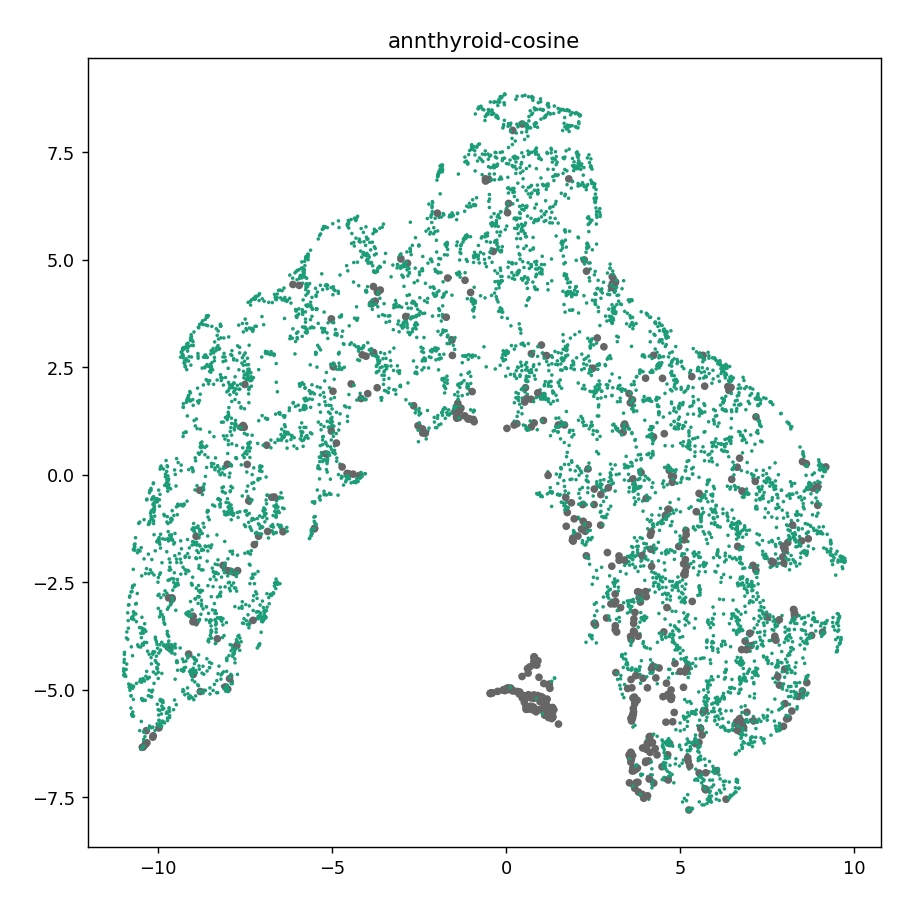
\includegraphics[width=2in]{images/umaps/annthyroid-cosine-umap2d.png}
    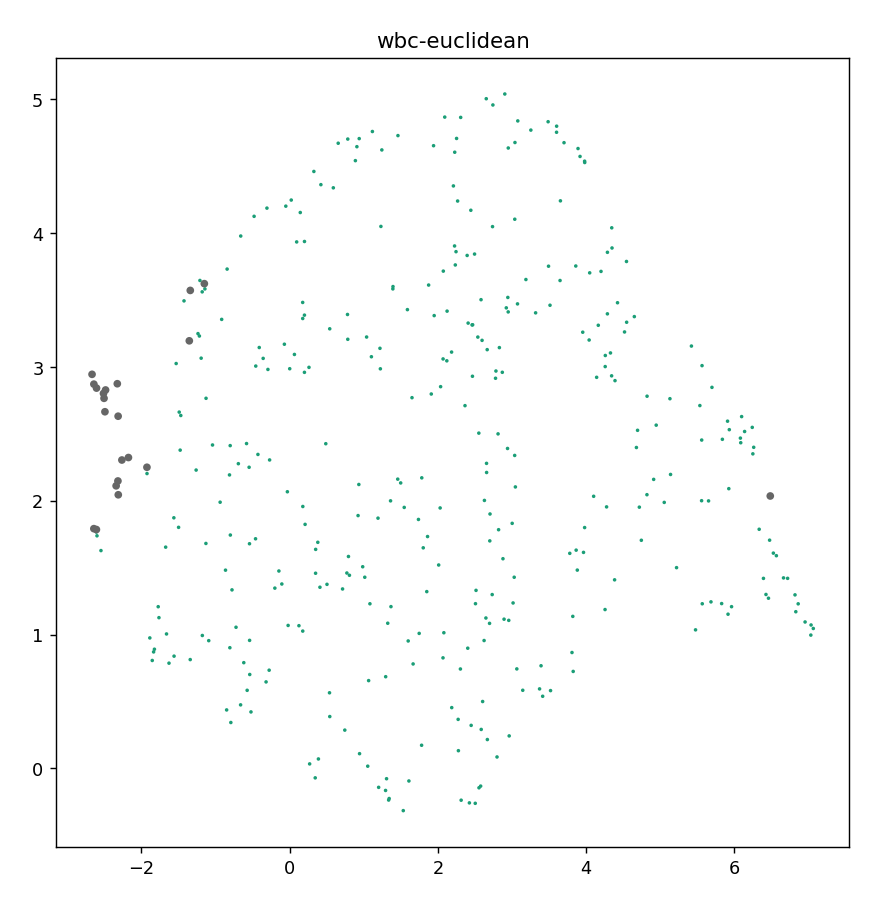
\includegraphics[width=2in]{images/umaps/wbc-euclidean-umap2d.png}
    \caption{UMAP projection of Annthyroid (left) and WBC (right). Anomalies are in gray. Note that for Annthyroid, while there is a cluster of anomalies off the main manifold, many anomalies are distributed throughout the manifold. For WBC, the anomalies tend to be at the edge of the manifold.}
    \label{fig:conclusions:umap-embeddings}
\end{figure*}

One current limitation in CHAODA is that the depth of the cluster tree at which anomaly detection performs best is not the same for every dataset;
thus, our results could be seen as ``cherry-picking'' from a scattershot approach.
The optimal depth varies because as depth increases, the induced graph ``shatters'', i.e.\ the number of components in the graph approaches the number of clusters in the graph.
Future work should explore optimal stopping criteria so that we can automate stopping just before the graph shatters.
Fortunately, as shown in Figures, for most datasets, performance is not overly sensitive to the choice of depth, especially for the Parent-Child algorithm.
For now we can treat depth as a hyperparameter to all of the methods described, but a detailed analysis of possible stopping criteria for clustering depth will likely reveal automatic methods to find the optimal depth.

% TODO: Need to look at local fractal dimension, or volume ratios, vs. optimal depth. Ideally we can say something like:
% The strong correlation between local fractal dimension and optimal tree depth suggests a guideline for determining an optimal tree depth directly from the data.

The choice of distance function also has a significant impact on anomaly-detection performance.
In this case, domain knowledge is likely the best way to determine the distance function of choice.
Future work will seek to explore a more diverse collection of domain-appropriate distance functions, such as Wasserstein distance on images, Levenshtein edit distance on strings, and Jaccard Index on the Maximal Common Sub-Graph of molecular structures. 

% TODO: Have we proved this?
% Say something about applying CHAODA for inputs to an ANN, in particular detecting just-off-manifold malicious inputs, like the school bus / ostrich example.

In conclusion, we have demonstrated that by learning approximate manifolds, we can exploit the embedded knowledge to implement simple algorithms capable of outperforming other state-of-the-art approaches to anomaly detection.

\section{Acknowledgements}
\label{sec:acknowledgements}

The authors would like to thank the members of CSC 592 - Algorithms for Big Data for helpful feedback and discussions.
% We have been Clearly Hoping that Our Work Detects Anomalies.


\bibliography{references}


\end{document}
